\section{Künstliches Neuronales Netz}
\rhead{Künstliches Neuronales Netz}

Künstliche neuronale Netze (KNN) stellen eine Möglichkeit des maschinellen Lernens dar, welche vom Hirn inspiriert wurde.
Ein KNN besteht aus verschiedenen Neuronen, welche hierarchisch in sogenannten Layern angeordnet werden (vgl. Abbildung \ref{fig:neuralnet}).
Jeder Eingangswert $x_i$ zu einem Neuron wird mit einem Faktor $w_i$ multipliziert.
Alle gewichteten Eingänge werden zusammen mit einem Schwellenwert $b$ addiert.
Diese Summe wird danach durch eine nichtlineare Aktivierungsfunktion $H$ aktiviert und bildet so den Ausgang $y$
\begin{equation} \label{eq:neuron}
y=H\left(\sum_{i} x_i w_i+b\right).
\end{equation}
Die Nichtlinearität ist entscheidend um nichtlineare Probleme lösen zu können.
Der Aufbau eines Neuron ist in Abbildung \ref{fig:neuron} gezeigt. 

\begin{figure}
	\centering
	\def\layersep{2.5cm}

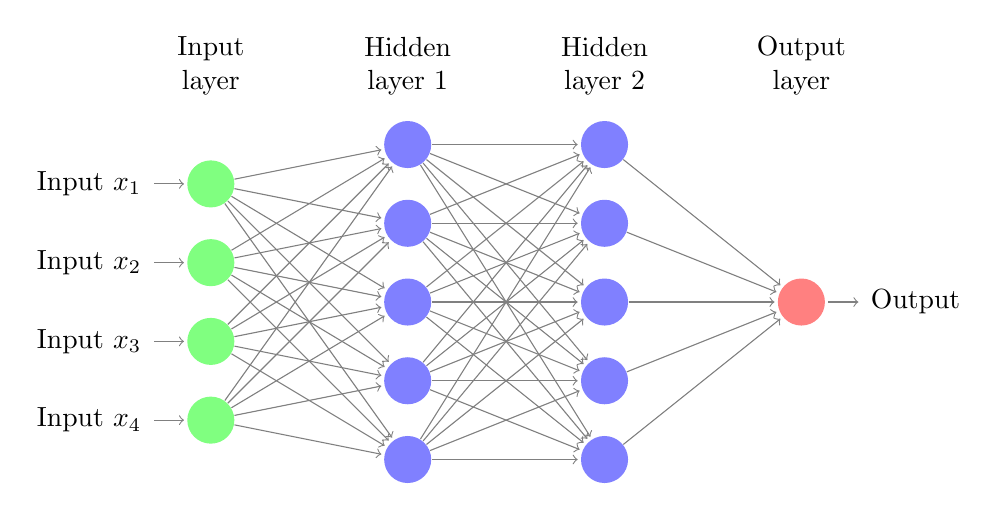
\begin{tikzpicture}[shorten >=1pt,->,draw=black!50, node distance=\layersep]
\tikzstyle{every pin edge}=[<-,shorten <=1pt]
\tikzstyle{neuron}=[circle,fill=black!25,minimum size=17pt,inner sep=0pt]
\tikzstyle{input neuron}=[neuron, fill=green!50];
\tikzstyle{output neuron}=[neuron, fill=red!50];
\tikzstyle{hidden neuron}=[neuron, fill=blue!50];
\tikzstyle{hidden neuron 2}=[neuron, fill=blue!50];
\tikzstyle{annot} = [text width=4em, text centered]

% Draw the input layer nodes
\foreach \name / \y in {1,...,4}
	\node[input neuron, pin=left:Input $x_{\y}$] (I-\name) at (0,-\y) {};

% Draw the hidden layer 1 nodes
\foreach \name / \y in {1,...,5}
	\path[yshift=0.5cm]
		node[hidden neuron] (H-\name) at (\layersep,-\y cm) {};

% Draw the hidden layer 2 nodes
\foreach \name / \y in {1,...,5}
	\path[yshift=0.5cm]
		node[hidden neuron 2] (H2-\name) at (2*\layersep,-\y cm) {};

% Draw the output layer node
\node[output neuron,pin={[pin edge={->}]right:Output}, right of=H2-3] (O) {};

% Connect every node in the input layer with every node in the
% hidden layer.
\foreach \source in {1,...,4}
	\foreach \dest in {1,...,5}
		\path (I-\source) edge (H-\dest);
\foreach \source in {1,...,5}
	\foreach \dest in {1,...,5}
		\path (H-\source) edge (H2-\dest);

% Connect every node in the hidden layer with the output layer
\foreach \source in {1,...,5}
	\path (H2-\source) edge (O);

% Annotate the layers
\node[annot,above of=H-1, node distance=1cm] (hl) {Hidden layer 1};
\node[annot,left of=hl] {Input layer};
\node[annot,right of=hl] (hl2) {Hidden layer 2};
\node[annot,right of=hl2] {Output layer};
\end{tikzpicture}

	\caption{Aufbau eines neuronalen Netzes mit zwei hidden Layern (blau) und einem output Layer (rot). Die blauen und roten Kreise stellen also die Neuronen dar, die Grünen sind der Input.}
	\label{fig:neuralnet}
\end{figure}

\begin{figure}
	\centering
	\tikzstyle{inputNode}=[draw,circle,minimum size=10pt,inner sep=0pt]
\tikzstyle{stateTransition}=[->, thick]
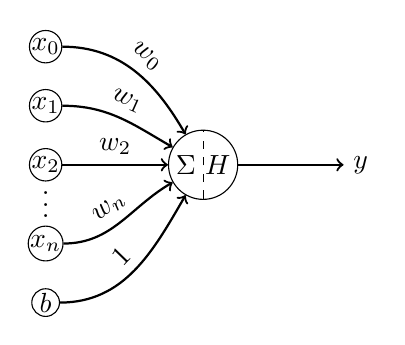
\begin{tikzpicture}
\node[draw,circle,minimum size=25pt,inner sep=0pt] (x) at (0,0) {$\Sigma$ $H$};
\node[] (y) at (2,0) {$y$};

\node[inputNode] (x0) at (-2, 1.5) {$x_0$};
\node[inputNode] (x1) at (-2, 0.75) {$x_1$};
\node[inputNode] (x2) at (-2, 0) {$x_2$};
\node[inputNode] (xn) at (-2, -1.0) {$x_n$};
\node[inputNode] (b) at (-2, -1.75) {$b$};

\draw[stateTransition] (x0) to[out=0,in=120] node [midway, sloped, above] {$w_0$} (x);
\draw[stateTransition] (x1) to[out=0,in=150] node [midway, sloped, above] {$w_1$} (x);
\draw[stateTransition] (x2) to[out=0,in=180] node [midway, sloped, above] {$w_2$} (x);
\draw[stateTransition] (xn) to[out=0,in=210] node [midway, sloped, above] {$w_n$} (x);
\draw[stateTransition] (b) to[out=0,in=240] node [midway, sloped, above] {$1$}(x);
\draw[stateTransition] (x) to node [midway,above=-0.1cm] {}(y);
\draw[dashed] (0,-0.43) -- (0,0.43);
\node (dots) at (-2, -0.4) {$\vdots$};
\end{tikzpicture}
	\caption{Aufbau eines Neurons äquivalent zur Gleichung \ref{eq:neuron}.}
	\label{fig:neuron}
\end{figure}

\subsection{Convolutional Neural Nets}

Eine Unterkategorie der KNNs stellen die Convolutional Neural Nets (CNN) dar.
Wie der Name schon sagt, spielen dabei Faltungen eine wichtige Rolle.
Bevor die normalen KNN Layer kommen, werden Bilddaten üblicherweise zuerst von einigen Faltungslayern vorverarbeitet.
Die Idee dazu kommt von der klassischen Bildverarbeitung, wo häufig Faltungskernel verwendet werden um ein Bild zu filtern oder Features zu erkennen.
Bei einem CNN werden diese Kernel nicht vom Ingenieur bestimmt, sondern während Trainings durch den Algorithmus gelernt.  
Die gelernten Gewichte (Kernels) haben an jeder Position der Faltung die selben Werte, sind also Translationsinvariant.
Diese Eigenschaft ist entscheidend, da sie einerseits die Anzahl zu lernender Gewichte extrem reduziert und andererseits die Generalisierung fördert.
Solche CNNs zeigen extrem gute Resultate in der Bildverarbeitung, speziell im Bereich der Klassifizierung von Bildern (z.B. Erkennen von Katzen).
Wie eine zweidimensionale Faltung funktioniert ist in Abbildung \ref{fig:2dconv} gezeigt.

\begin{figure}
	\centering
	\usetikzlibrary{matrix, positioning}
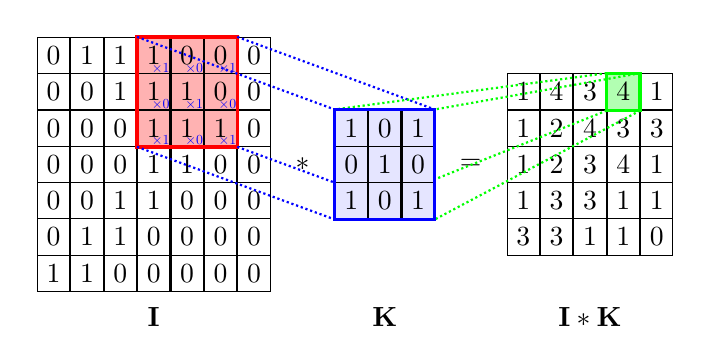
\begin{tikzpicture}

	\matrix (mtr) [matrix of nodes,row sep=-\pgflinewidth, nodes={draw}]
	{
		0 & 1 & 1 & |[fill=red!30]| 1 & |[fill=red!30]| 0 & |[fill=red!30]| 0 & 0\\
		0 & 0 & 1 & |[fill=red!30]| 1 & |[fill=red!30]| 1 & |[fill=red!30]| 0 & 0\\
		0 & 0 & 0 & |[fill=red!30]| 1 & |[fill=red!30]| 1 & |[fill=red!30]| 1 & 0\\
		0 & 0 & 0 & 1 & 1 & 0 & 0\\
		0 & 0 & 1 & 1 & 0 & 0 & 0\\
		0 & 1 & 1 & 0 & 0 & 0 & 0\\
		1 & 1 & 0 & 0 & 0 & 0 & 0\\
	};

	\draw[very thick, red] (mtr-1-4.north west) rectangle (mtr-3-6.south east);

	\node [below= of mtr-5-4.south] (lm) {$\bf I$};

	\node[right = 0.2em of mtr] (str) {$*$};

	\matrix (K) [right=0.2em of str,matrix of nodes,row sep=-\pgflinewidth, nodes={draw, fill=blue!30}]
	{
		1 & 0 & 1 \\
		0 & 1 & 0 \\
		1 & 0 & 1 \\
	};
	\node [below = of K-3-2.south] (lk) {$\bf K$};

	\node [right = 0.2em of K] (eq) {$=$};

	\matrix (ret) [right=0.2em of eq,matrix of nodes,row sep=-\pgflinewidth, nodes={draw}]
	{
		1 & 4 & 3 & |[fill=green!30]| 4 & 1\\
		1 & 2 & 4 & 3 & 3\\
		1 & 2 & 3 & 4 & 1\\
		1 & 3 & 3 & 1 & 1\\
		3 & 3 & 1 & 1 & 0\\
	};
	\node [below = of ret-4-3.south] (lim) {${\bf I} * {\bf K}$};

	\draw[very thick, green] (ret-1-4.north west) rectangle (ret-1-4.south east);

	\draw[densely dotted, blue, thick] (mtr-1-4.north west) -- (K-1-1.north west);
	\draw[densely dotted, blue, thick] (mtr-3-4.south west) -- (K-3-1.south west);
	\draw[densely dotted, blue, thick] (mtr-1-6.north east) -- (K-1-3.north east);
	\draw[densely dotted, blue, thick] (mtr-3-6.south east) -- (K-3-3.south east);

	\draw[densely dotted, green, thick] (ret-1-4.north west) -- (K-1-1.north west);
	\draw[densely dotted, green, thick] (ret-1-4.south west) -- (K-3-1.south west);
	\draw[densely dotted, green, thick] (ret-1-4.north east) -- (K-1-3.north east);
	\draw[densely dotted, green, thick] (ret-1-4.south east) -- (K-3-3.south east);

	\matrix (K) [right=0.2em of str,matrix of nodes,row sep=-\pgflinewidth, nodes={draw, fill=blue!10}]
	{
		1 & 0 & 1 \\
		0 & 1 & 0 \\
		1 & 0 & 1 \\
	};

	\draw[very thick, blue] (K-1-1.north west) rectangle (K-3-3.south east);

	\node[anchor=south east, inner sep=0.01em, blue] at (mtr-1-4.south east) (xx) {\scalebox{.5}{$\times 1$}};
	\node[anchor=south east, inner sep=0.01em, blue] at (mtr-1-5.south east) (xx) {\scalebox{.5}{$\times 0$}};
	\node[anchor=south east, inner sep=0.01em, blue] at (mtr-1-6.south east) (xx) {\scalebox{.5}{$\times 1$}};
	\node[anchor=south east, inner sep=0.01em, blue] at (mtr-2-4.south east) (xx) {\scalebox{.5}{$\times 0$}};
	\node[anchor=south east, inner sep=0.01em, blue] at (mtr-2-5.south east) (xx) {\scalebox{.5}{$\times 1$}};
	\node[anchor=south east, inner sep=0.01em, blue] at (mtr-2-6.south east) (xx) {\scalebox{.5}{$\times 0$}};
	\node[anchor=south east, inner sep=0.01em, blue] at (mtr-3-4.south east) (xx) {\scalebox{.5}{$\times 1$}};
	\node[anchor=south east, inner sep=0.01em, blue] at (mtr-3-5.south east) (xx) {\scalebox{.5}{$\times 0$}};
	\node[anchor=south east, inner sep=0.01em, blue] at (mtr-3-6.south east) (xx) {\scalebox{.5}{$\times 1$}};

\end{tikzpicture}
	\caption{Darstellung einer zweidimensionalen Faltung des Bildes $I$ mit dem Kernel $K$.}
	\label{fig:2dconv}
\end{figure}

Anhand von der Bildverarbeitung kann man den Unterschied von KNNs und CNNs gut erklären.
Bei einem KNN wird jedes Pixel mit jedem Neuron verbunden und für jede dieser Verbindungen wird ein eigenes Gewicht gelernt.
Beim CNN hingegen wird ein einzelner Kernel gelernt, welcher dann translationsinvariant auf das ganze Bild angewendet wird.
Als Beispiel nehmen wir einen ersten Layer von $256$ Neuronen, ein Eingangsbild der Grösse $128\times128$ und eine Kernelgrösse von $3\times3$.
Damit erhalten wir beim KNN	$256 \cdot 128 \cdot 128 = 4'227'072$ Gewichte welche gelernt werden müssen.
Beim CNN hingegen genügen $256 \cdot 3 \cdot 3 = 2'304$ Gewichte.

Die zweidimensionale Wavelet-Transformation kann auch als Faltung des Bildes mit dem Wavelet (Kernel) interpretiert werden.
Dabei werden allerdings nicht mehr alle kontinuierlichen Grössen des Wavelets berücksichtigt, sondern nur noch eine diskrete Anzahl.
Da KNNs (und CNNs) vom Hirn inspirierte Algorithmen darstellen und die Bildvorverarbeitung im Hirn als Gabor-Wavelet-Transformation modelliert werden kann, drängt sich daher eine Kombination dieser beiden Konzepte auf.

Eine offensichtliche Idee ist dabei das Vorverabeiten der Bilder mithilfe von Gabor-Wavelets.
Diese vorverarbeiteten Bilder können dann als Input in das CNN verwendet werden und sollten gute Resultate zeigen, analog zum menschlichen Hirn.
Ob diese theoretischen Ideen auch praktisch anwendbar sind, soll ein Versuch zeigen.

\subsection{Versuch}

Das Ziel des Versuches ist es, zu zeigen ob Gabor-Wavelets wirklich eine Berechtigung im Zusammenhang mit CNNs haben.
Zwei verschiedene Dinge sollen überprüft werden:
\begin{enumerate}
	\item Ist eine vorverarbeitung mittels Gabor-Kerneln sinnvoll?
	\item Lernt ein CNN Kernels welche Ähnlichkeiten zu den Gabor-Kerneln besitzen?
\end{enumerate}
Um diese Ziele zu erreichen wurde ein Versuch durchgeführt, bei welchem der CIFAR-10 \cite{paper:cifar10} Datensatz klassifiziert werden soll.
Beim CIFAR-10 Datensatz handelt es sich um $32 \times 32$ Pixel grosse farbige Bilder,welche zu zehn verschiedenen Klassen gehören (z.B. Flugzeug, Vogel, etc.).
Der Datensatz umfasst dabei 50'000 Trainings- und 10'000 Testbilder.
Ein Beispiel jeder Klasse ist in Abbildung \ref{fig:cifar10} gezeigt.
Der CIFAR-10 Datensatz wurde gewählt da er ziemlich bekannt ist, Beispielarchitekturen verfügbar sind und relativ schwierig zu lösen ist.
Die Schwierigkeit ist wichtig um überhaupt einen Unterschied in der Genauigkeit feststellen zu können (bei 99\% Genauigkeit sieht man keine grossen Verbesserungen mehr).

\begin{figure}
	\centering
	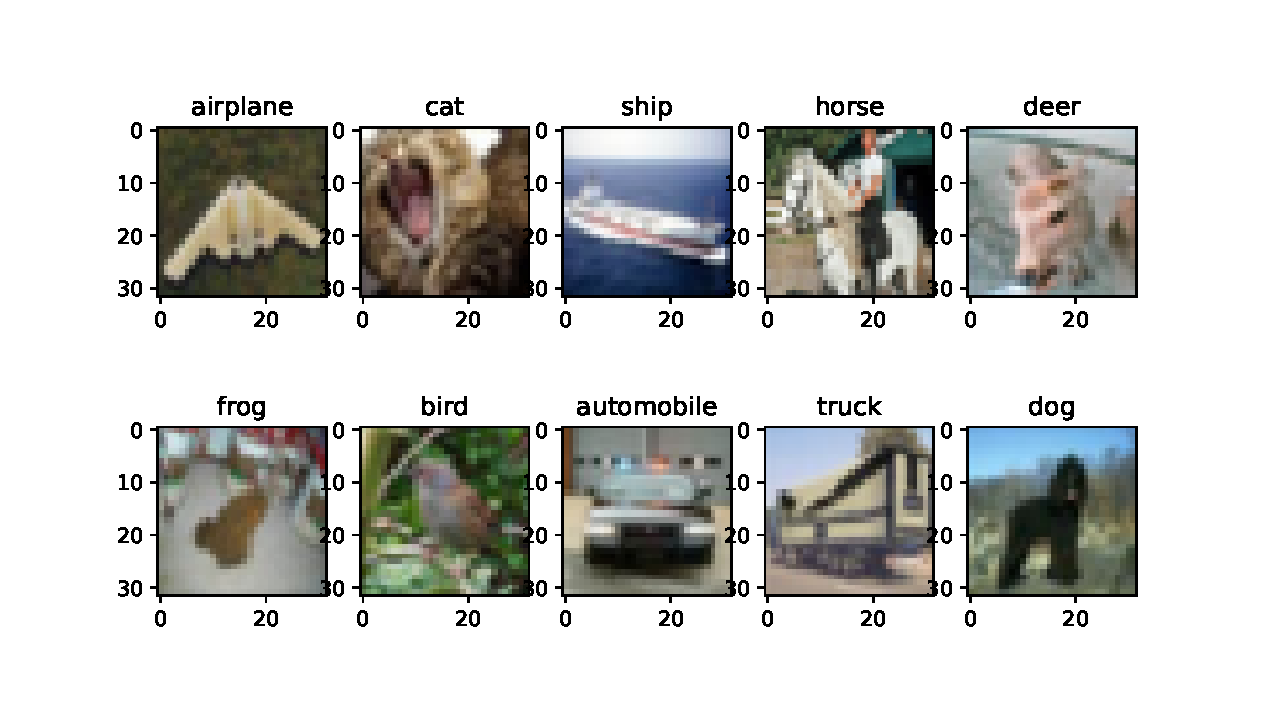
\includegraphics[width=0.6\linewidth, trim=0 60 0 40, clip]{./papers/visuell/images/cifar10}
	\caption{Die zehn verschiedenen Klassen des CIFAR-10 Datensatzes.}
	\label{fig:cifar10}
\end{figure}

Die Architektur des CNNs ist inspiriert von einem Artikel über CIFAR-10 \cite{online:cifar10}.
Implementiert wurde das gesamte Projekt mit Python und Tensorflow.

Der erste Convolutional-Layer besteht aus $64$ verschiedenen $9 \times 9$ Kerneln, welche entweder gelernt werden oder als Gabor-Kernels gesetzt werden.
Also wird das Netzwerk zwei mal trainiert, einmal mit einem fixen ersten Layer (Gabor-Layer) und einmal mit einem lernbaren ersten Layer.
Die Variante mit Gabor-Layer stellt dem Netzwerk weniger Freiheitsgrade zur Verfügung und sollte theoretisch ein schlechteres Resultat zeigen.
Da wir aber vermuten das ein Gabor-Layer eine optimale Vorverarbeitung darstellt, sollten die Gabor-Kernels besser Resultate als die selbst gelernten zeigen.

Nach dem ersten Layer folgen drei weitere Convolutional-Layer, bevor am Ende fünf Fully-Connected-Layer (normale KNN-Layer) das Resultat ausgeben.
Die genaue Architektur ist in Tabelle \ref{table:architecture} gezeigt.
Die Bilder werden zuerst in schwarzweiss Bilder umgewandelt, damit die Gabor-Variante keinen Nachteil bekommt.
Der Nachteil würde entstehen, da das Netzwerk für jede Farbe andere Features lernen könnte, wohingegen die Gabor-Variante auf allen Farben die gleichen Kernels benutzen würde. 

\begin{table}
	\centering
	\begin{tabular}{|c|c|c|}
		\hline
		Layer & Kernelgrösse & Ausgangsgrösse \\ 
		\hline \hline
		Input & - & $32 \times 32 \times 1$ \\ 
		\hline 
		Conv1 & $9 \times 9$ &  $32 \times 32 \times 64$\\ 
		\hline 
		Conv2 & $3 \times 3$ &  $32 \times 32 \times 128$\\  
		\hline 
		Pool2 & - &  $16 \times 16 \times 128$\\ 
		\hline 
		Conv3 & $3 \times 3$ & $16 \times 16 \times 256$\\ 
		\hline 
		Pool3 & - &  $8 \times 8 \times 256$\\ 
		\hline 
		Conv4 & $3 \times 3$ & $8 \times 8 \times 512$\\ 
		\hline 
		Pool4 & - &  $4 \times 4 \times 512$\\ 
		\hline 
		Flatten & - & $ 8192 $ \\ 
		\hline 
		FC1 & - & $ 128 $ \\ 
		\hline 
		FC2 & - & $ 256 $ \\
		\hline 
		FC3 & - & $ 512 $ \\  
		\hline 
		FC4 & - & $ 1024 $ \\ 
		\hline 
		Softmax & - & $ 10 $ \\ 
		\hline
	\end{tabular} 
	\caption{Unsere Netzwerk-Architektur. Der erste Layer (Conv1) wird bei der Gabor-Variante fix gesetzt und nicht gelernt. Nach jedem Convolutional- und Fully-Connected-Layer wird eine Batch-Normalization durchgeführt. Die Aktivierungsfunktion ist immer ReLu, ausser beim Softmax-Output.}
	\label{table:architecture}
\end{table}


